\documentclass{beamer}

\usepackage{iftex}

\iftutex
% For LuaTeX or XeTeX Use Google's
% OpenType Noto fonts for typesetting
% Russian text
\usepackage{fontspec}
\defaultfontfeatures{Ligatures={TeX}}
\setmainfont{Noto Serif}
\setsansfont{Noto Sans}
\setmonofont{Noto Sans Mono}

\else
% For pdfTeX we must use old
% 8-bit font technologies
\usepackage[T2A]{fontenc}
\fi

% Hyphenation rules
\usepackage{hyphenat}
\usepackage[english, russian]{babel}

% More styles for bullets
\usepackage{pifont}

% Using listings to highlight code
\usepackage{listings}

% Information to be included in the title page:
\title{
    Neuro-semantic industrial control
    \ifdefined\tagversion
        \newline
        \newline
        v\tagversion
    \fi}
\author{Иванюк Д.~С.}
\institute{Савушкин продукт}
\date{\today}

% TikZ is probably the most complex and powerful tool to create graphic elements in LaTeX.
\usepackage{tikz}

\addtobeamertemplate{navigation symbols}{}{%
    \usebeamerfont{footline}%
    \usebeamercolor[fg]{footline}%
    \hspace{1em}%
    \insertframenumber/\inserttotalframenumber
}

\begin{document}

\usetikzlibrary{positioning,fit,calc} % used for the efficient working of the positioning system

\tikzset{block/.style={draw, thick, text width=1cm, minimum height=.5cm, align=center},
    % the align command is used to align the block diagram at the center
    % the height command adjust the height of the block diagram
    % here block diagram refers to the whole diagram, not the single block
    % the thick command here signifies the border of all the blocks used inside the block diagram. You can change it to thin command if you want the thin edge of the blocks
    line/.style={-latex}   % the lesser the width the greater will be the diagram window
}

\frame{\titlepage}

\begin{frame}
    \frametitle{Содержание}
    \tableofcontents
\end{frame}

\section{Нейроуправление}
 {
  \begin{frame}
    \frametitle{Нейроуправление}

    \tikzset{
        box/.style={
                % The shape:
                rectangle,
                % The size:
                minimum size=20mm,
                % The border:
                very thick,
                draw=red!50!black!50,         % 50% red and 50% black,
                % and that mixed with 50% white
                % The filling:
                top color=white,              % a shading that is white at the top...
                bottom color=red!50!black!20, % and something else at the bottom
                % Font
                font=\itshape,
                align=center}}

    \tikzset{big_arrow/.style={-{Stealth[length=5mm, width=4mm]}}}

    \centering
    \usetikzlibrary {positioning,shapes.misc,calc,arrows.meta,arrows}
    \begin{tikzpicture}[
            right1/.style={to path={-- ++(4,0) |- (\tikztotarget)}},
            left1/.style={to path={-- ++(-4,0) |- (\tikztotarget)}}]
        \node (o1)   [box]                        {Объект\\управления};
        \node (u1)   [below=of o1,align=center]   {$\mathbf{ U(t) }$\\Эффективность};
        \node (c1)   [box,below=of u1]            {Управляющее\\устройство\\(контроллер)};

        \node (control) [right=of c1,align=center]  {$\mathbf{ u(t) }$\\Управление};
        \node (sensors) [left=of c1,align=center]   {$\mathbf{ X(t) }$\\Показания датчиков};

        \path {
            (o1)            edge[very thick]                     (u1)
            (u1)            edge[very thick, big_arrow]          (c1)
            ($ (c1.east) $) edge[very thick, big_arrow, right1]  ($ (o1.east) $)
            ($ (o1.west) $) edge[very thick, big_arrow, left1]   ($ (c1.west) $) };
    \end{tikzpicture}

  \end{frame}

  \begin{frame}{Разработанный нейро-ПИД-контроллер}
    \begin{figure}
        \centering
        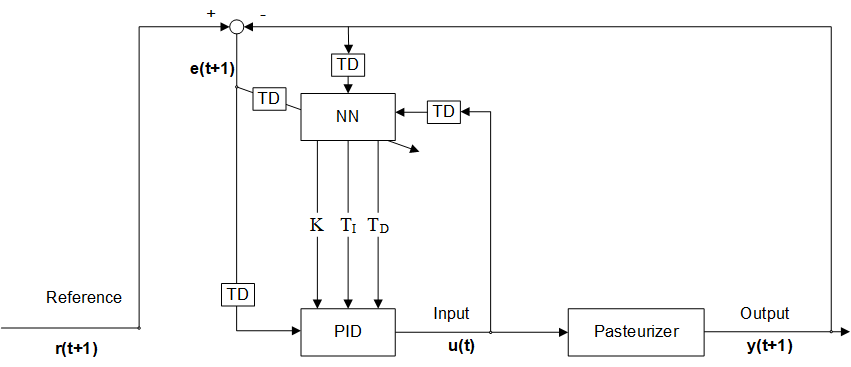
\includegraphics[width=\textwidth]{images/developed-NN.png}
    \end{figure}
  \end{frame}

  \begin{frame}{Настройщик ПИД}
    \begin{figure}
        \centering
        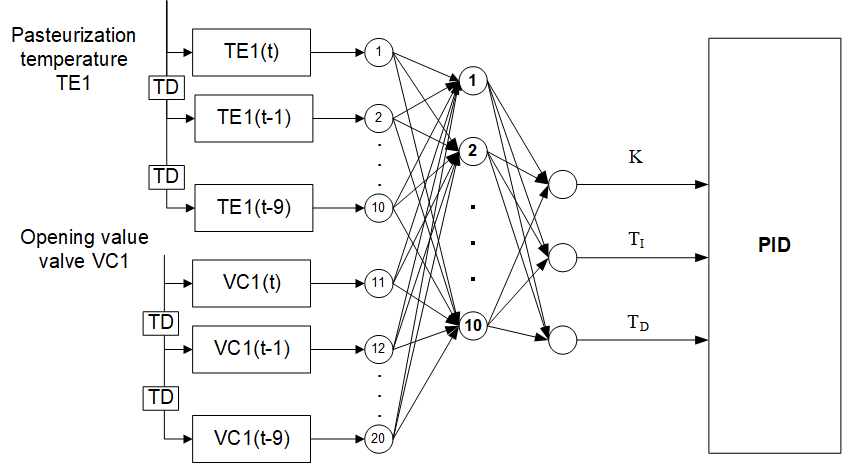
\includegraphics[width=\textwidth]{images/neuro-adjuster-PID.png}
    \end{figure}
  \end{frame}

  \begin{frame}
    \frametitle{Нейронные сети}

    \centering
    \begin{tikzpicture}
        \node[rectangle, fill=black, text=white, minimum height=1cm] (n) {neural network};
        \node[left=of n] (in) {inputs};
        \node[right=of n] (out) {outputs};

        \draw[line] (in)--(n);
        \draw[line] (n)--(out);
    \end{tikzpicture}

\end{frame}
 }

 \section{Семантические технологии}
 {
    \begin{frame}{S88}
        \begin{itemize}
            \item \textit{ANSI/ISA-88.00.01-2010}, Batch Control –- Part 1: Models and Terminology;
            \item \textit{ISA-88.00.02-2001}, Batch Control –- Part 2: Data Structures and Guidelines for Languages;
            \item \textit{ANSI/ISA-TR88.00.02-2015}, Machine and Unit States: An implementation example of \textit{ANSI/ISA-88.00.01};
            \item \textit{ISA-88.00.03-2003}, Batch Control –- Part 3: General and Site Recipe Models and Representation;
            \item \textit{ISA-TR88.0.03-1996}, Possible Recipe Procedure Presentation Formats;
            \item \textit{ANSI/ISA-88.00.04-2006}, Batch Control –- Part 4: Batch Production Records;
            \item \textit{ISA-TR88.95.01-2008}, Using ISA-88 and ISA-95 Together;
            \item \textit{IEC 61512-1}, The European version approved in 1997, based on the older version \textit{ISA-88.01-1995};
            \item \textit{GOST R IEC 61512-1-2016} -- Russian version of the standard, identical to \textit{IEC 61512-1}.
        \end{itemize}
    \end{frame}

    \begin{frame}{S95}
        \begin{itemize}
            \item \textit {ANSI/ISA-95.00.01-2010}, Enterprise-Control System Integration -- Part 1: Models and Terminology;
            \item \textit {ANSI/ISA-95.00.02-2018}, Enterprise-Control System Integration -- Part 2: Objects and Attributes for Enterprise-Control System Integration;
            \item \textit {ANSI/ISA-95.00.03-2013}, Enterprise-Control System Integration -- Part 3: Activity Models of Manufacturing Operations Management;
            \item \textit {ANSI/ISA-95.00.04-2018}, Enterprise-Control System Integration -- Part 4: Objects and Attributes for Manufacturing Operations Management Integration;
        \end{itemize}
    \end{frame}

    \begin{frame}{S95}
        \begin{itemize}
            \item \textit {ANSI/ISA-95.00.05-2018}, Enterprise-Control System Integration -- Part 5: Business-to-Manufacturing Transactions;
            \item \textit {ANSI/ISA-95.00.06-2014}, Enterprise-Control System Integration -- Part 6: Messaging Service Model;
            \item \textit {ANSI/ISA-95.00.07-2017}, Enterprise-Control System Integration -- Part 7: Alias Service Model;
            \item \textit {ANSI/ISA-95.00.08-2020}, Enterprise-Control System Integration -– Part 8: Information Exchange Profiles.
        \end{itemize}
    \end{frame}

    \begin{frame}{ISA-5.1}
        \begin{itemize}
            \item \textit {ANSI/ISA-5.1-2022}, Instrumentation Symbols and Identification;
            \item \textit {ISA-5.9 working group}, Controller Algorithms and Performance;
            \item \textit {ISA-5.4}, Instrument Loop Diagrams;
            \item \textit {ISA-5.5-1985}, Graphic Symbols for Process Displays;
            \item \textit {ISA-5.6}, Documentation for Control Software Applications;
        \end{itemize}
    \end{frame}

    \begin{frame}{Устройства управления}
        \begin{figure}
            \centering
            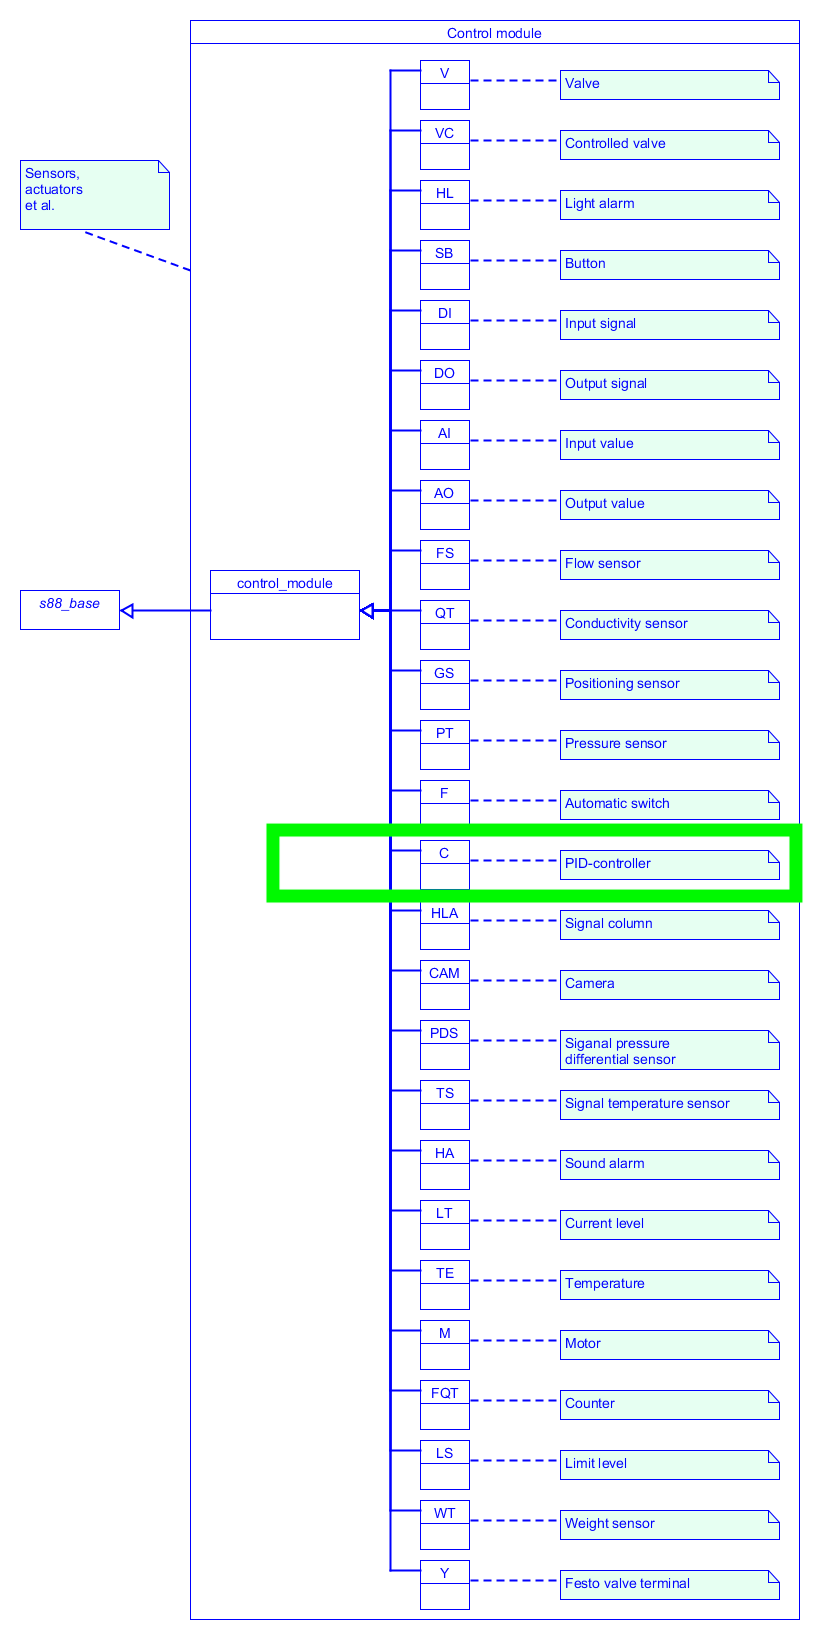
\includegraphics[width=0.7\textwidth]{images/control-modules-s88.png}
        \end{figure}
      \end{frame}
 }

 \section{Нейро + семантическое управление на основе OSTIS}
 {
    \begin{frame}{OSTIS в управлении}
        \begin{figure}
            \centering
            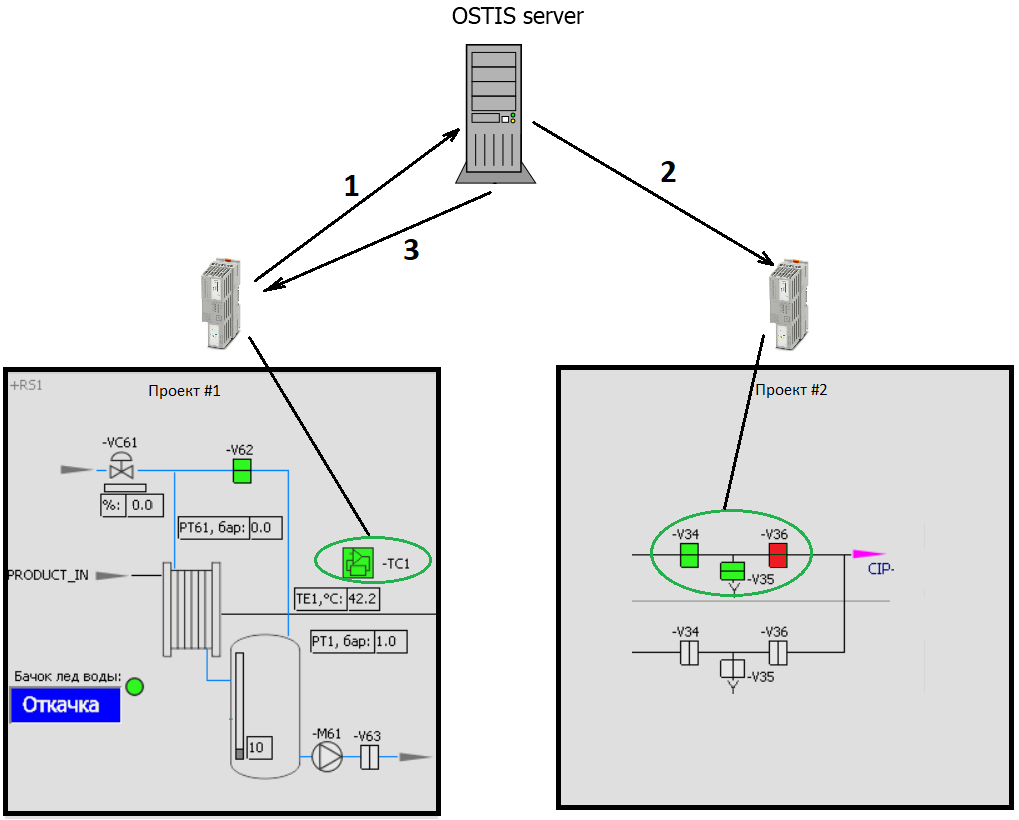
\includegraphics[width=\textwidth]{images/OSTIS-in-control.png}
        \end{figure}
      \end{frame}
 }

 \section{Выводы}
 {
 }

\end{document}
